
\section{Introduction}

\begin{frame}{Genetic Algorithms using Neural Networks}

  \begin{itemize}
    \item Population with individuals
    \item Individuals are candidate solutions
    \item Neural networks as candidate solutions
    \item Continuous procreation
  \end{itemize}
%  introduction of some sort
%  what did we work with (briefly)
%  why did we do it? (motivation)
%  how did we end up working with diversity?
\end{frame}

\begin{frame}{Fun and exciting}
  \begin{figure}
    \centering
    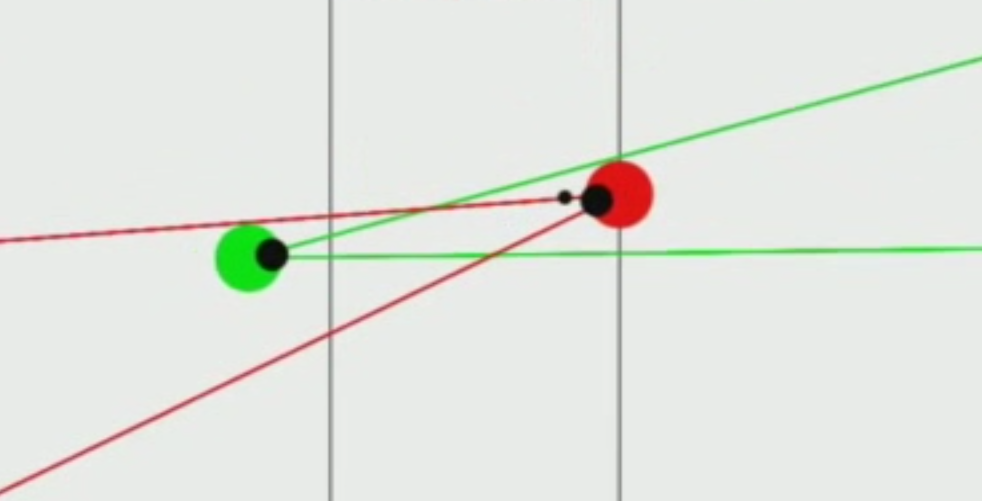
\includegraphics[width=250px]{elias/images/sniper.png}
    \caption{\url{youtube.com/watch?v=u2t77mQmJiY}}
    %by Ding Nicolas
  \end{figure}
\end{frame}

%\begin{frame}{Motivation}
%  \begin{figure}
%    \centering
%    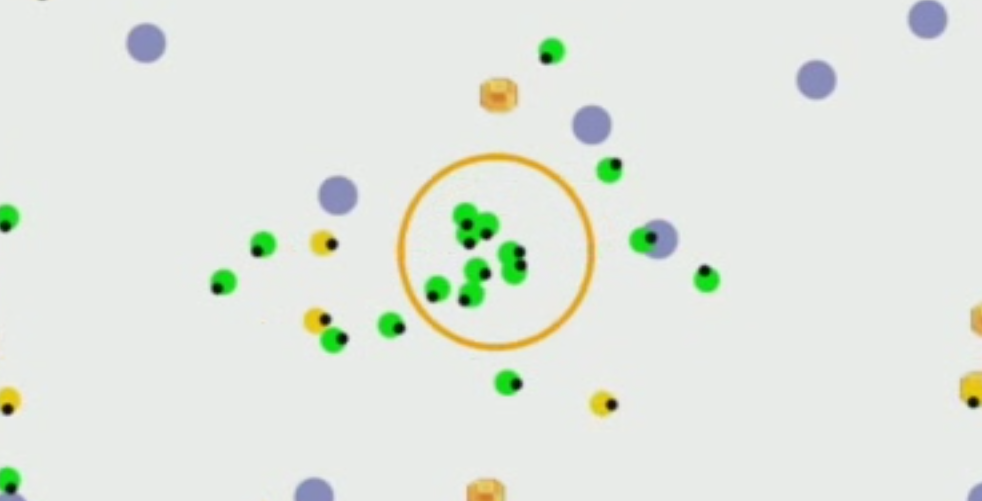
\includegraphics[width=250px]{elias/images/swarm.png}
%    \caption{\url{youtube.com/watch?v=Iv_Fy6Urik4}}
    %by Ding Nicolas
%  \end{figure}
%\end{frame}

\begin{frame}{Useful and serious}
  \begin{figure}
    \centering
    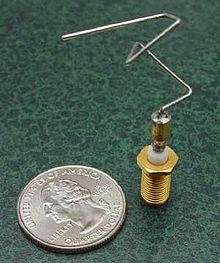
\includegraphics[height=100px]{elias/images/antenna.jpg}
    \caption{\url{en.wikipedia.org/wiki/genetic_algorithm}}
  \end{figure}
  \begin{itemize}
    \item Measuring diversity?
  \end{itemize}
\end{frame}

%\section{Candidate Solutions}

\begin{frame}{Representing Candidate Solutions}
    \begin{center}
      \inputresizeto{0.5\textwidth}{elias/images/neuralnetwork}
    \end{center}
  %  picture of use of neural networks
      \begin{itemize}
        \item Static network structure
        \item Weights represent the network as bit strings
        \item Straightforward manipulation
      \end{itemize}
    %  bit strings as chromosomes to be manipulated
\end{frame}

\begin{frame}{Assessing Candidate Solutions}
  \begin{itemize}
    \item How good is a candidate solution? How fit is it?
    \item Which conditions are important to observe?
    \item Defining a fitness function
  \end{itemize}
%  fitness functions and importance
\end{frame}

\section{Existing Diversity Measures}

\begin{frame}{Existing Diversity Measures}
  \begin{itemize}
    \item Genotypic diversity measure (genetic make-up)
    \item Phenotypic diversity measure (behaviour/fitness)
  \end{itemize}
\end{frame}

\begin{frame}{Genotypic measures}
  \begin{figure*}
  \begin{subfigure}{0.5\textwidth}
    \centering
    \inputresizeto{0.5\linewidth}{drawings/eqnetworks/eqnetworks3}
    \caption{An artificial neural network with connections and weights.}\label{fig:eqnetwork}
  \end{subfigure}
  \begin{subfigure}{0.5\textwidth}
    \centering
    \inputresizeto{0.5\linewidth}{drawings/eqnetworks/eqnetworks4}
    \caption{An artificial neural network equivalent to \cref{fig:eqnetwork}.}\label{fig:eqnetwork2}
  \end{subfigure}
  \caption{Networks with same phenotype, but different genotypes. The binary representation assumes that each weight is represented by four bits.}\label{fig:entire-eqnetwork}
\end{figure*}


  \begin{itemize}
    \item Hamming distance of 6
    \item Levenschtein distance of 6
    \item Genotypically diverse
    \item Phenotypically equal
  \end{itemize}
%  illustration of the workings of hamming distance
\end{frame}

\begin{frame}{Fitness-based phenotypic measure}
  \begin{figure}
    \centering
    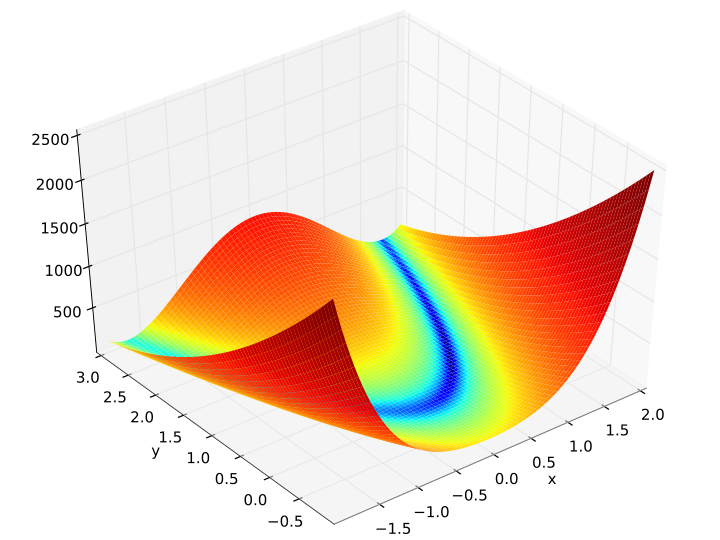
\includegraphics[height=150px]{elias/images/elevation.png}
    \caption{\url{en.wikipedia.org/wiki/rosenbrock_function}}
  \end{figure}
\end{frame}

\begin{frame}{What should be measured?}
  \begin{itemize}
    \item What about the actual behaviour?
    \item Which behaviour do candidate solutions have?
    \item Categorize according to behaviour
  \end{itemize}
\end{frame}

%\begin{frame}{What are they good for?}
%  \begin{itemize}
%    \item Cheap evaluation
%  \end{itemize}
%\end{frame}

